\chapter{Objetivos y Metodología}\label{chap:objetivos}

En este capítulo, se presentarán los objetivos generales y específicos del trabajo, junto con los criterios definidos para comprobar su cumplimiento. 
Posteriormente, se describirá la metodología adoptada para el desarrollo del proyecto, así como la planificación prevista, los riesgos identificados y los recursos necesarios para su realización.

\section{Objetivos Generales}\label{sec:objgenerales}

El objetivo general es desarrollar y evaluar un asistente institucional, capaz de consultar documentación interna mediante un sistema \textit{Retrieval-Augmented Generation} (RAG) y de apoyar acciones operativas mediante herramientas integradas, con el fin de mejorar su utilidad en un entorno controlado.

A mayores se persigue analizar en qué medida una mejora del componente de recuperación, basada en recuperación híbrida y \textit{reranking}, produce un efecto observable sobre la calidad de la evidencia recuperada y de las respuestas generadas, en comparación con un \textit{baseline} de recuperación semántica simple.

\section{Objetivos Específicos}\label{sec:objespecificos}

Para alcanzar el objetivo general, se plantean los siguientes objetivos específicos:

\begin{enumerate}
    \item \textbf{Identificar} los requisitos funcionales y no funcionales de un asistente institucional privado, atendiendo a aspectos como consulta documental, fundamentación de respuestas, trazabilidad, control del flujo y uso supervisado de herramientas.

    \item \textbf{Diseñar} una arquitectura modular basada en un agente orquestador que coordine la recuperación de información, la generación de respuestas y la invocación de herramientas externas.

    \item \textbf{Desarrollar} un prototipo funcional capaz de procesar consultas en lenguaje natural sobre documentación interna y generar respuestas apoyadas en evidencia recuperada.

    \item \textbf{Integrar} una funcionalidad accionable basada en herramientas, centrada en la generación de correos electrónicos formales a partir de la información obtenida durante la consulta.

    \item \textbf{Establecer} un \textit{baseline} de recuperación basado en búsqueda semántica simple para disponer de una referencia inicial de funcionamiento.

    \item \textbf{Implementar} una variante mejorada del componente de recuperación de información mediante una estrategia de recuperación híbrida y \textit{reranking}.

    \item \textbf{Definir} un conjunto de casos de prueba representativos del dominio institucional, incluyendo consultas informativas, consultas sobre procedimientos y consultas orientadas a acción.

    \item \textbf{Comparar} el rendimiento del \textit{baseline} y de la variante mejorada mediante métricas de recuperación, fundamentación de respuestas, utilidad de la salida generada y coste temporal del sistema.

    \item \textbf{Evaluar} a través de métricas en qué medida la mejora introducida en el componente de recuperación repercute en la calidad global del asistente y en su capacidad para ofrecer respuestas útiles y operativamente aprovechables.

    \item \textbf{Analizar} las fortalezas, limitaciones y posibles líneas de mejora de la solución propuesta en el contexto de asistentes institucionales privados y uso de herramientas.
\end{enumerate}

\section{Criterios de comprobación de los objetivos}\label{sec:criterios}

Con el fin de que los objetivos anteriores puedan verificarse de forma objetiva, se emplearán los siguientes criterios de comprobación:

\begin{itemize}
    \item El conjunto de evaluación deberá contener al menos 25 casos de prueba representativos del dominio.
    
    \item El prototipo deberá ser capaz de generar una respuesta para, al menos, el 90\% de los casos de prueba definidos.
    
    \item En los casos orientados a acción, el sistema deberá generar correos para, al menos, el 90\% de las consultas correspondientes.
    
    \item La comparación entre el \textit{baseline} y la variante mejorada se realizará mediante métricas de recuperación como Recall@5 y MRR@5.
    
    \item Se considerará que la mejora propuesta produce un efecto observable si la variante mejorada obtiene, al menos, una mejora de 3 puntos porcentuales en Recall@5 o una mejora relativa del 5\% en MRR@5 respecto al \textit{baseline}. 
    En ambos casos, el valor @5 indica que la evaluación se realiza sobre los cinco primeros documentos recuperados por el sistema para cada consulta.
    
    \item Se considerará satisfactorio que al menos el 75\% de las respuestas generadas por la variante mejorada se apoyen de forma clara en los documentos recuperados.
        
    \item El coste temporal del sistema se medirá mediante la latencia media por consulta, procurando que la variante mejorada no incremente dicho tiempo en más de un 50\% respecto al \textit{baseline}.
\end{itemize}

\section{Metodología del trabajo}\label{sec:metodologia}

En el desarrollo de este se adoptará una metodología ágil basada en Scrum, al considerarse un enfoque adecuado para organizar un proyecto tecnológico con una parte aplicada y otra parte evaluativa. 
Esta elección se justifica por su flexibilidad, su carácter iterativo y su capacidad para adaptarse a cambios en los requisitos, en las decisiones de diseño o en los resultados obtenidos durante la implementación y la evaluación del sistema.

En este caso, el trabajo no consiste únicamente en desarrollar un prototipo funcional, sino también en analizar comparativamente el comportamiento de distintas configuraciones del componente de recuperación de información. 
Por ello, Scrum se empleará como marco de organización y seguimiento del desarrollo, permitiendo dividir el trabajo en incrementos manejables, revisar periódicamente el progreso y ajustar decisiones conforme avance el proyecto.

\subsection{Scrum}

Scrum es un marco de trabajo ágil orientado al desarrollo incremental de productos. 
Su funcionamiento se basa en iteraciones cortas y planificadas, denominadas \textit{sprints}, al final de las cuales se obtiene un incremento funcional del sistema. 
Este enfoque resulta apropiado, ya que permite avanzar de forma progresiva desde la definición del problema hasta la implementación del prototipo y su evaluación experimental.

\subsection{Roles}

Dado el contexto académico del trabajo, los roles de Scrum se adaptarán de forma simplificada:

\begin{itemize}
    \item \textbf{Product Owner}: asumido por la dirección, al encargarse de supervisar el enfoque general del trabajo, validar su orientación y priorizar los elementos más relevantes del proyecto.
    \item \textbf{Scrum Master}: también asumido de forma parcial por la dirección, en la medida en que orienta el desarrollo, ayuda a resolver bloqueos y supervisa la coherencia metodológica del trabajo.
    \item \textbf{Equipo de desarrollo}: asumido por la estudiante, responsable del análisis, diseño, implementación, experimentación y redacción de la memoria.
\end{itemize}

\subsection{Artefactos}

Los principales artefactos de trabajo serán los siguientes:

\begin{itemize}
    \item \textbf{Product Backlog}: listado priorizado de tareas y objetivos del proyecto, incluyendo decisiones de arquitectura, preparación documental, implementación de componentes, diseño de experimentos y redacción.
    \item \textbf{Sprint Backlog}: subconjunto de tareas seleccionadas para cada sprint.
    \item \textbf{Incremento}: resultado funcional o evaluable obtenido al final de cada sprint, como puede ser una primera arquitectura definida, un \textit{baseline} operativo o una versión mejorada del sistema.
\end{itemize}

\subsection{Eventos}

El trabajo se organizará mediante los eventos habituales de Scrum, adaptados a un proyecto individual:

\begin{itemize}
    \item \textbf{Sprint Planning}: definición de las tareas a abordar en cada iteración.
    \item \textbf{Seguimiento}: revisión periódica del progreso, dificultades encontradas y ajustes necesarios.
    \item \textbf{Sprint Review}: revisión del resultado obtenido al final de cada sprint.
    \item \textbf{Sprint Retrospective}: valoración de los aspectos que han funcionado correctamente y de los elementos a mejorar en la siguiente iteración.
\end{itemize}

\subsection{Adaptación al proyecto}

Aunque Scrum se concibe habitualmente para equipos de desarrollo, su estructura puede adaptarse a un trabajo individual. 
Los \textit{sprints} no se orientarán únicamente a implementar funcionalidades, sino también a producir resultados parciales verificables.

De este modo, la metodología de desarrollo permitirá combinar dos dimensiones del trabajo: por una parte, la construcción iterativa del asistente institucional privado; por otra, la comparación entre un \textit{baseline} de recuperación semántica y una variante mejorada basada en recuperación híbrida y \textit{reranking}. 

\section{Riesgos y planes de contingencia}\label{sec:riesgos}

Durante el desarrollo resulta necesario identificar posibles riesgos técnicos, metodológicos y de planificación que puedan afectar al alcance, a la calidad de la solución o al calendario previsto. 
Dado que el proyecto combina implementación de un prototipo funcional con una evaluación experimental comparativa, la gestión de riesgos adquiere especial relevancia para asegurar la viabilidad del trabajo.

A continuación, se describen los principales riesgos identificados y las medidas de contingencia previstas para reducir su impacto:

\begin{enumerate}
    \item \textbf{Dificultades en la integración de componentes heterogéneos.}  
    La integración entre el modelo de lenguaje, el componente de recuperación, la base documental y la funcionalidad accionable puede presentar incompatibilidades técnicas o requerir más esfuerzo de implementación del previsto.  
    Como plan de contingencia, se priorizará una arquitectura modular y desacoplada, permitiendo validar cada componente por separado antes de su integración completa. 

    \item \textbf{Calidad insuficiente de la base documental o del conjunto de evaluación.}  
    El rendimiento del asistente depende en gran medida de la calidad del corpus documental y de la representatividad de los casos de prueba. Un conjunto poco adecuado podría dificultar tanto el funcionamiento del sistema como la evaluación de la mejora propuesta.  
    Como medida de contingencia, se realizará una selección y revisión temprana del corpus y de las consultas de prueba, garantizando que cubran los escenarios principales del dominio.

    \item \textbf{Resultados experimentales poco concluyentes.}  
    Existe la posibilidad de que la mejora basada en recuperación híbrida y \textit{reranking} no produzca diferencias suficientemente claras respecto al \textit{baseline}, o que dichas diferencias no sean tan amplias como se esperaba inicialmente.  
    Como plan de contingencia, el trabajo no se orientará a demostrar una mejora absoluta, sino a realizar una comparación controlada y rigurosa entre ambas configuraciones. 

    \item \textbf{Incremento excesivo de la latencia del sistema.}  
    La incorporación de una segunda etapa de recuperación o de un mecanismo de \textit{reranking} puede aumentar el tiempo de respuesta del asistente y comprometer su utilidad práctica como prototipo.  
    Para mitigar este riesgo, se medirá la latencia desde las primeras versiones funcionales y se limitará el número de documentos candidatos o el coste de los modelos auxiliares en caso necesario.

    \item \textbf{Cambios en el alcance o en las decisiones técnicas durante el desarrollo.}  
    Como sucede en muchos proyectos de desarrollo e investigación aplicada, algunas decisiones inicialmente previstas pueden necesitar ajustes conforme avance la implementación o la evaluación.  
    Como medida de contingencia, se adoptará una planificación iterativa basada en Scrum, de forma que cada sprint permita revisar el estado del trabajo, reordenar prioridades y acotar el alcance sin perder coherencia con los objetivos definidos.

    \item \textbf{Retrasos en el calendario previsto.}  
    La simultaneidad entre implementación, experimentación y redacción de la memoria puede provocar desviaciones temporales respecto a la planificación inicial.  
    Para reducir este riesgo, se organizará el trabajo en incrementos parciales y se reservará una fase final específica para revisión, análisis de resultados y redacción. 

    \item \textbf{Limitaciones derivadas del carácter individual del proyecto.}  
    Al tratarse de un TFM desarrollado de forma individual, tanto el análisis como la implementación, la evaluación y la documentación recaen sobre una única persona, lo que puede ralentizar el avance en fases de mayor carga técnica.  
    Como contingencia, se mantendrá una planificación realista, con objetivos acotados y verificables, evitando incorporar funcionalidades adicionales que no resulten imprescindibles para demostrar la contribución principal del trabajo.
\end{enumerate}


\section{Planificación del trabajo}\label{sec:planificacion}

De manera general, cada sprint tendrá una duración aproximada de entre dos y tres semanas, como se muestra en la Figura~\ref{fig:gantt}, aunque esta distribución podrá adaptarse en función de la complejidad real de las tareas y de las incidencias surgidas durante el desarrollo. 
Al final de cada iteración se realizará una revisión del avance conseguido y una replanificación de las tareas pendientes, con el fin de mantener el proyecto alineado con los objetivos establecidos.

\subsection{Sprint 1: análisis y definición del problema}

En esta primera fase se concretará el alcance del trabajo, se revisará el estado del arte ya recopilado y se terminarán de definir los requisitos funcionales y no funcionales del asistente institucional privado. 
Asimismo, se delimitará el caso de uso principal, se identificarán las capacidades mínimas del prototipo y se establecerán los criterios de evaluación que se utilizarán en la parte experimental.

Durante esta fase también se seleccionarán las herramientas y tecnologías necesarias para implementar el sistema, así como el enfoque general de la arquitectura.

\subsection{Sprint 2: diseño de la arquitectura y preparación del entorno de trabajo}

El primer sprint estará centrado en el diseño técnico del sistema. En esta etapa se definirá la arquitectura modular del asistente, identificando los componentes principales, sus responsabilidades y el flujo de interacción entre ellos. 
En particular, se detallará el papel del agente orquestador, el componente de recuperación documental, el modelo generativo y la funcionalidad de herramienta integrada.

Además, se preparará el entorno de desarrollo, se seleccionará o estructurará el corpus documental inicial y se organizará el material necesario para la construcción posterior del prototipo.

\subsection{Sprint 3: implementación del \textit{baseline} del asistente}

En este sprint se desarrollará una primera versión funcional del sistema, que actuará como \textit{baseline}. 
Esta configuración inicial permitirá procesar consultas en lenguaje natural, recuperar documentos relevantes mediante búsqueda semántica simple y generar respuestas apoyadas en la evidencia recuperada.

El objetivo de esta fase será disponer de una referencia operativa sobre la que poder comparar posteriormente la mejora investigadora del trabajo. 
Al finalizar este sprint deberá existir una primera versión ejecutable del asistente, aunque todavía limitada a su funcionalidad esencial.

\subsection{Sprint 4: integración de la funcionalidad accionable}

Una vez disponible el \textit{baseline}, el siguiente sprint se centrará en ampliar el sistema con una capacidad accionable. 
En concreto, se integrará la generación de borradores de correos electrónicos formales a partir de la consulta del usuario y de la información recuperada desde la base documental.

Esta fase permitirá que el asistente no solo responda preguntas, sino que también apoye una actuación posterior útil dentro del entorno institucional. 
Al finalizar este sprint, el prototipo deberá ser capaz de producir una salida operativa básica en los casos orientados a acción.

\subsection{Sprint 5: implementación de la mejora del componente de recuperación de información}

El cuarto sprint estará orientado a la principal aportación experimental del TFM. 
En esta etapa se implementará una variante mejorada del componente de recuperación de información basada en recuperación híbrida y \textit{reranking}, manteniendo la posibilidad de compararla con el \textit{baseline} definido anteriormente.
El objetivo será introducir una mejora concreta y controlada sobre el proceso de recuperación documental, sin modificar de forma radical el resto del sistema. 

\subsection{Sprint 6: diseño de la evaluación y comparación experimental}

En este sprint se preparará y ejecutará la evaluación comparativa entre el \textit{baseline} y la variante mejorada. 
Para ello, se terminará de construir el conjunto de casos de prueba, se definirán las rúbricas de evaluación manual y se recogerán las métricas seleccionadas para el análisis.

La comparación se centrará en dimensiones como la calidad de la recuperación, la fundamentación de las respuestas, la utilidad de los borradores generados y el coste temporal del sistema. 
Esta fase permitirá disponer de resultados cuantitativos con los que analizar el impacto real de la mejora propuesta.

\subsection{Sprint 7: Revisión final, análisis de resultados y redacción de la memoria}

La última fase del trabajo se dedicará a consolidar los resultados obtenidos, interpretar los datos recogidos durante la evaluación y redactar la memoria final del TFM. 
También se revisará el grado de cumplimiento de los objetivos planteados y se identificarán las principales limitaciones del sistema, así como posibles líneas de mejora o ampliación futura.
Esta etapa incluirá además la revisión formal de la memoria.

\begin{figure}[H]
    \centering
    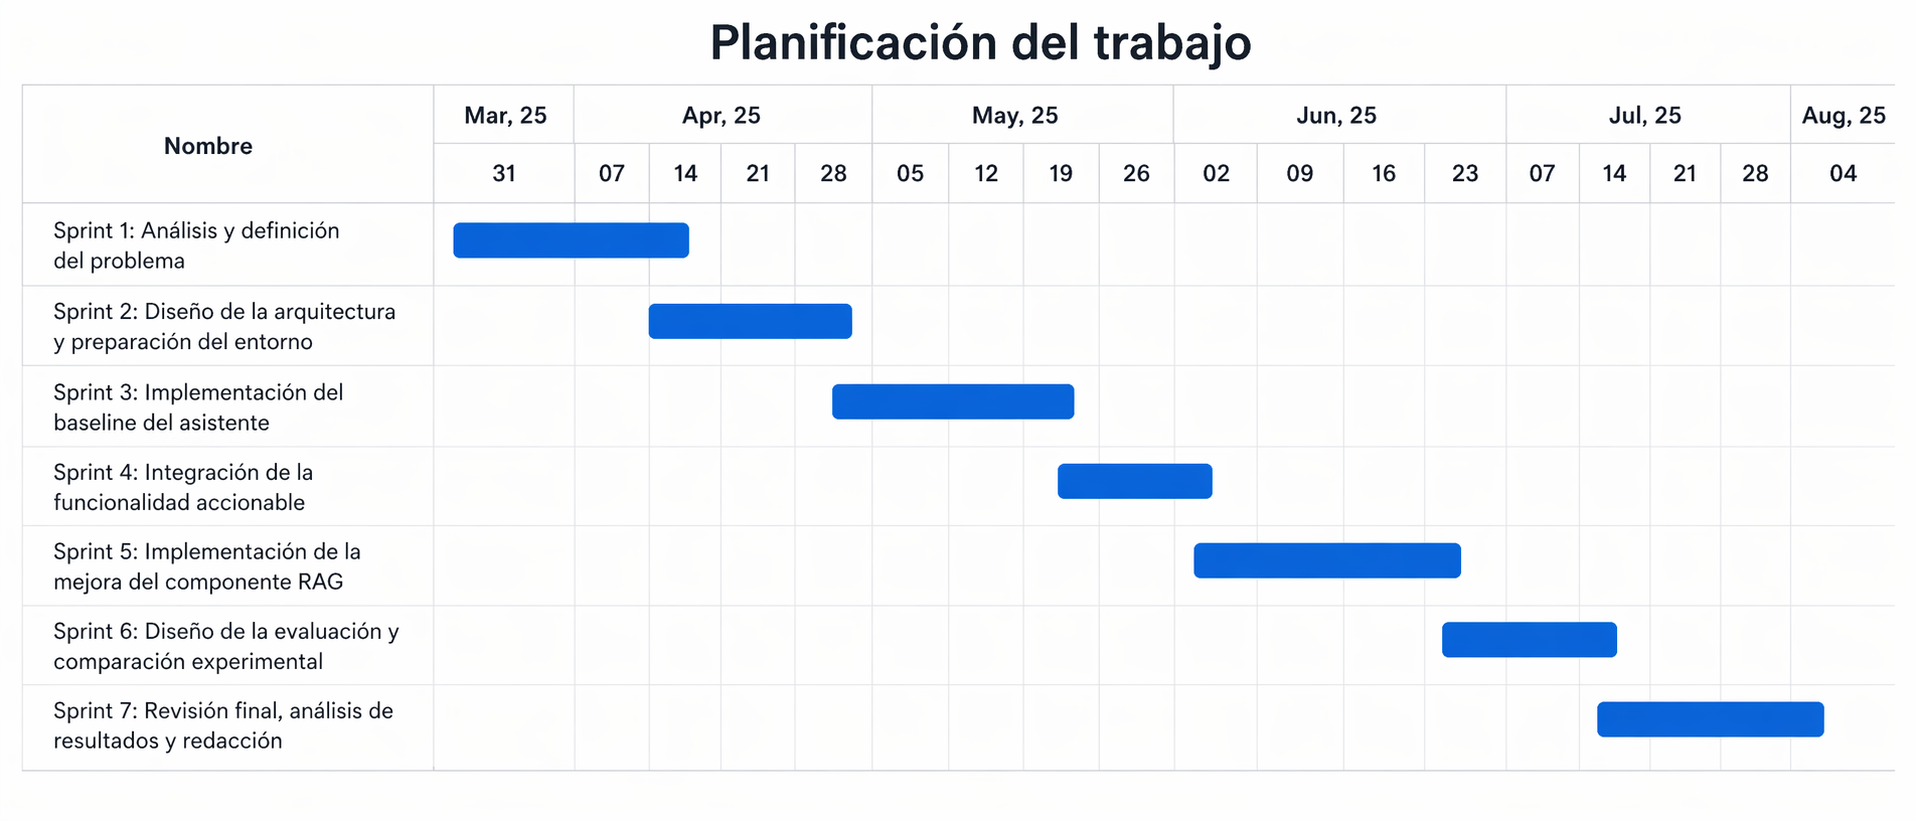
\includegraphics[width=1\textwidth]{contenido/imagenes/Gantt.png}
    \caption{Diagrama de Gantt con la planificación temporal del trabajo.}
    \label{fig:gantt}
\end{figure}

\section{Recursos y costes}\label{sec:recursos}

En esta sección se describen los recursos necesarios y se realiza una estimación orientativa de sus costes. 
Dado que se trata de un proyecto académico desarrollado de forma individual, la mayor parte del esfuerzo recae en la estudiante, mientras que la dirección del TFM asume funciones de supervisión, revisión y seguimiento. 

\subsection{Recursos humanos}

Los recursos humanos considerados para el desarrollo del proyecto son los siguientes:

\begin{itemize}
    \item \textbf{Dirección del TFM}: responsable de orientar el trabajo, revisar su evolución, validar las decisiones principales y supervisar la coherencia metodológica y académica del proyecto.
    
    \item \textbf{Estudiante}: responsable del análisis del problema, diseño de la arquitectura, implementación del prototipo, preparación del conjunto de evaluación, ejecución de los experimentos, análisis de resultados y redacción de la memoria final.
\end{itemize}

Aunque el proyecto es realizado por una única persona, desde el punto de vista de la estimación puede considerarse que la estudiante asume varias funciones de forma simultánea, entre ellas las de analista, desarrolladora e investigadora aplicada.

\subsection{Recursos técnicos}

Para el desarrollo del TFM se requerirán los siguientes recursos técnicos:

\begin{itemize}
    \item Ordenador personal para desarrollo, pruebas y redacción de la memoria.
    \item Entorno de programación y herramientas de desarrollo para la implementación del prototipo.
    \item Herramientas de edición y documentación para la elaboración de diagramas, esquemas y memoria.
    \item Servicios o librerías necesarios para la implementación del sistema RAG, la integración del modelo generativo y el procesamiento documental.
    \item Herramientas de evaluación y análisis de resultados.
\end{itemize}

En términos generales, se priorizará el uso de herramientas gratuitas, académicas o ya disponibles en el entorno de trabajo, por lo que no se prevé un coste material elevado asociado al proyecto. 
En caso de utilizar servicios externos de pago, estos quedarán limitados a un uso puntual o experimental.

\subsection{Estimación de dedicación}

La siguiente tabla recoge una estimación orientativa de las horas de trabajo necesarias para desarrollar el proyecto:

\begin{table}[H]
\centering
\begin{tabular}{lccc}
\toprule
\textbf{Rol} & \textbf{Horas proyecto} & \textbf{Horas memoria} & \textbf{Total horas} \\
\midrule
Estudiante & 300 & 120 & 420 \\
Dirección del TFM & 20 & 10 & 30 \\
\bottomrule
\end{tabular}
\caption{Estimación de horas dedicadas al proyecto.}
\label{tab:horas_proyecto}
\end{table}

La dedicación principal corresponde a la estudiante, ya que asume tanto el desarrollo técnico del prototipo como la parte experimental y documental del trabajo. 
En cambio, la dirección del TFM participa de manera periódica mediante reuniones de seguimiento, revisión de avances y supervisión de la memoria.

\subsection{Estimación de costes}

A efectos de estimación, se asigna un coste por hora orientativo a cada uno de los roles considerados. Estos valores no deben interpretarse como costes contractuales reales, sino como una aproximación académica al esfuerzo invertido en el proyecto.

\begin{table}[H]
\centering
\begin{tabular}{lccc}
\toprule
\textbf{Rol} & \textbf{Total horas} & \textbf{Coste/hora (€)} & \textbf{Coste total (€)} \\
\midrule
Estudiante & 420 & 25 & 10.500 \\
Dirección del TFM & 30 & 35 & 1.050 \\
\midrule
\textbf{Total} & \textbf{450} & -- & \textbf{11.550} \\
\bottomrule
\end{tabular}
\caption{Estimación orientativa de costes humanos del proyecto.}
\label{tab:costes_proyecto}
\end{table}

Por tanto, el coste total estimado del proyecto, considerando únicamente los recursos humanos, sería de 11.550\,€. 
Esta cifra representa una valoración aproximada del esfuerzo necesario para desarrollar el asistente, implementar la mejora experimental propuesta y documentar adecuadamente el trabajo realizado.

